% Modified 31 Oct 2005:  Conditioning fallacy alluded to.
% This chapter has been modified on 6-4-05.
% There are two \choice
\pagestyle{headings}
\chapter{Probability} \label{chp 3}

\section{Sample Spaces \& Events}

Suppose the outcome of an experiment is uncertain, but we can represent the collection of all possible outcomes by writing it as a set.

\begin{definition} A set which represents the collection of all possible outcomes of an experiment is known as a \newterm{sample space}\index{Sample Space}, typically denoted $\Omega$.
\end{definition}

Specifying a concrete representation of the set of all outcomes of an experiment will often clarify the context of a problem and eliminate many potential sources of confusion.

\begin{example}Consider a single roll of a single six-sided die. In this experiment, there are six possible outcomes, corresponding to the six distinct faces of the die. Thus, we can take $\Omega = \{1,2,3,4,5,6\}$.
\end{example}

\begin{example}\label{BreakingStrength}Consider measuring the breaking strength (in Newtons) of a plank of wood. If we have no information about the size or shape of the plank, or about the precision with which the breaking strength will be measured, we should allow any positive real value. Thus, $\Omega = \{x \in \mathbb{R} \, | \, x \geq 0\}$.\end{example}

\begin{example}Suppose that a coin is flipped, and then a marble is drawn from an urn which contains black, white, and grey marbles. In this scenario, we could take $\Omega = \{HB,HW,HG,TB,TW,TG\}$, using $HB$ to represent flipping a head and drawing a black marble, $HW$ to represent flipping a head and drawing a white marble, and so on. \end{example}

\begin{example}\label{FlipUntilTail}Suppose you play a game where a coin is flipped repeatedly until the first tail appears. We could take $\Omega = \{T, HT, HHT, HHHT, HHHHT, \, \dots\, \}$, the set of all finite sequences of zero or more $H$'s followed by a single $T$.  \end{example}

As a sample space is a set, it can be countable or uncountable. We'll see later on in the course that the tools of calculus will come to our aid when dealing with probability problems that involve uncountable sample spaces.

The choice of sample space depends on the experiment and on what question the experimenters are trying to answer. If we roll a pair of dice, we might use the sample space $\Omega = \{2,3,4,\,\dots\,,11,12\}$ to count the sum of the two resulting values, or $\Omega = \{(1,1),(1,2),(2,1),(2,2),\,\dots\,,(5,6),(6,5),(6,6)\}$ to distinguish the dice and represent the value on each.

One big advantage of this larger sample space is that each of the outcomes is \emx{equally likely}. Imagine one die is red and the other is blue (the colours of the dice certainly won't influence the probabilities in this context). If neither die has any bias, then when the pair is rolled, each die is equally likely to land with any of its faces up. The red die showing 2 and blue showing 5 is as likely as the red die showing 6 and blue showing 6, and so on. In other words, each ordered pair of outcomes $(m,n)$ for $1 \leq m \leq 6$ and $1 \leq n \leq 6$ is as likely as any other.

If we write the number showing on the red die across the top row, the number showing on the blue die down the left column, and the sum of the two results in a table, we obtain the following.
{\small
\begin{center}\label{DiceRollTable}
\begin{tabular}{c|cccccc}
$_{B} \setminus ^R$ & 1 & 2 & 3 & 4 & 5 & 6 \\
\hline
1 & 2 & 3 & 4 & 5 & 6 & 7 \\
2 & 3 & 4 & 5 & 6 & 7 & 8 \\
3 & 4 & 5 & 6 & 7 & 8 & 9 \\
4 & 5 & 6 & 7 & 8 & 9 & $\!$10 \\
5 & 6 & 7 & 8 & 9 & $\!$10 & $\!$11 \\
6 & 7 & 8 & 9 & $\!$10 & $\!$11 & $\!$12 \\
\end{tabular}
\end{center}
}
Note that outcomes in the sample space $\Omega = \{2,3,4,\,\dots\,,11,12\}$ are not equally likely. There are six ordered pairs $(1,6)$, $(2,5)$, $(3,4)$, $(4,3)$, $(5,2)$, and $(6,1)$ which yield a sum of seven, while only the single pair $(1,1)$ gives a sum of two. This means rolling a sum of seven is six times more likely than rolling a sum of two.

\subsection*{Events in a Sample Space}

\begin{definition}
\newterm{Events}\index{Event} are subsets of a sample space in which we might be interested. We can describe an event using words or with more formal set notation.
\end{definition}

\begin{example}
Suppose we roll a single die. Let $\Omega = \{1,2,3,4,5,6\}$, let $E$ be the event `an even number is rolled' and let $G$ be the event `a number greater than four is rolled'. Then we can write $E = \{2,4,6\}$ and $G = \{5,6\}$.
\end{example}

\begin{example}\label{UnitSquare}
Consider a point selected at random inside a square with corners at $(0,0)$, $(1,0)$, $(0,1)$, and $(1,1)$. Let $\Omega = \{(x,y) \, | \, 0 \leq x \leq 1$ and $0 \leq y \leq 1\}$, and let $T$ be the event `the point is in the top half of the square'. Then using set notation we would write $T = \{(x,y) \, | \, 0 \leq x \leq 1$ and $0.5 \leq y \leq 1\}$.
\end{example}

Since events $A, B \subseteq \Omega$ are sets, we can form the events $A \cup B$ (at least one of $A$ and $B$ occur), $A \cap B$ (both $A$ and $B$ occur), and $A^{c}$ ($A$ does not occur). Te set operations allow us to build up complex events out of simpler pieces, or vice-versa, break a complex event into simpler pieces that are easier to deal with.

%Simple example using the operations with interpretation.

Let's return for a moment to rolling a pair of dice. If one of the dice shows a five, is it possible the sum is seven? Yes, since the outcomes $(5,2)$ and $(2,5)$ are elements of both events $F =$ `one of the dice shows five' and $S =$ `the sum is seven', that is, $F \cap S = \{(5,2), (2,5)\}$.

If one of the dice shows a five, is it possible the sum is three? No. If one die shows a five, the lowest possible sum is six. There are no elements common to the events $F =$ `one of the dice shows five' and $T =$ `the sum is three', that is, $F \cap S = \emptyset$.

\begin{definition}\label{mutuallyexclusive}\index{Mutually Exclusive Events}\index{Events!Mutually Exclusive}
Two events $A$ and $B$ in a sample space $\Omega$ are \newterm{mutually exclusive} if $A \cap B = \emptyset$, that is, if there are no outcomes in $\Omega$ where both events occur.
\end{definition}

\begin{example}
Consider an experiment where a coin is flipped, and then a die is rolled, and let $\Omega = \{H1,H2,H3,H4,H5,H6,T1,T2,T3,T4,T5,T6\}$. The events $H =$ `a head is flipped' and $E =$ `an even number is rolled' are not mutually exclusive, since $H \cap E = \{H2, H4, H6\}$.
\end{example}

\begin{example}
Suppose you're waiting for a bus, and you measure the number of seconds it takes for the bus to arrive. Let $E =$ `the bus arrives in under 3 minutes' and $F =$ `the bus takes more than 5 minutes to arrive'. Then $E$ and $F$ are mutually exclusive. Formally, let $\Omega = \{ x \in \mathbb{R} \, | \, x \geq 0\}$. In interval notation, we can write $E = [0,180)$ and $F = (300,\infty)$, then clearly $E \cap F = \emptyset$.
\end{example}

\section{Probability Models \& Probability Laws}

Consider a single roll of a fair six-sided die, and let $\Omega = \{1,2,3,4,5,6\}$. Since the die is fair, we should assign each of the six outcomes an equal probability of one-sixth.

If we want to find the probability any event $E \subseteq \Omega$ occurs, we can simply sum up the probabilities of each of the outcomes. If $E = \{2,4,6\}$ (an even number is rolled), then we write $P(E) = \frac{3}{6}$. To assign a probability to any event in this sample space, we can simply count up the number of outcomes in the event, and divide that number by six to obtain its probability.

\begin{definition}
A sample space $\Omega$, together with a way of assigning probabilities to all events $E \subset \Omega$, is known as a \newterm{probability model}\index{Probability Model}.
\end{definition}

\begin{example}
Describe a probability model on the sample space $\Omega = \{1,2,3,4,5,6\}$ for a six-sided die where each outcome is equally likely except for six, which is twice as likely as all the other outcomes.

Let $P(\{1\}) = q$. Then $P(\{6\}) = 2q$, and since it's certain that one of the six outcomes will occur,
$$\begin{aligned}
P(\{1,2,3,4,5,6\}) &= 1 \\
P(\{1\})+P(\{2\})+ \dots + P(\{5\})+P(\{6\}) &= 1 \\
q + q + \dots + q + 2q &= 1 \\
7q &= 1 \\
q &= \textstyle\frac{1}{7} \\
\end{aligned}$$

Therefore, the desired probability model assigns the outcomes one through five the probability $\frac{1}{7}$, and the outcome six the probability $\frac{2}{7}$.
\end{example}

\begin{keypoint}
For a \emx{countable} sample space, a probability model is an assignment of probabilities to the elements of $\Omega$. Once this is done, the probability of any event can be computed by summing the probabilities of the outcomes it contains. For an uncountable sample space, the situation is more subtle, as you'll see in the following example.
\end{keypoint}

\begin{example}\label{RandomPointInSquare}
Let $\Omega = \{(x,y) \,|\, 0 \leq x \leq 1 \text{ and } 0 \leq y \leq 1\}$, a unit square in $\mathbb{R}^2$. How can we describe a probability model in which a point in this unit square is selected at random?

Consider the smaller square $E = \{(x,y) \,|\, 0 \leq x \leq \frac{1}{2} \text{ and } 0 \leq y \leq \frac{1}{2}\}$ shaded below. Since this smaller square occupies one-quarter of the area, we should certainly have $P(E) = \frac{1}{4}$. 

\begin{center}
\begin{minipage}{1.6in}
\begin{center}
\begin{tikzpicture}[scale=0.7]
\draw (-1.5,-1.5) rectangle (1.5,1.5);
\draw (-1.5,-1.5) rectangle (0,0);
\fill [pattern=north east lines, pattern color=black] (-1.5,-1.5) rectangle (0,0);
\end{tikzpicture}
\end{center}
\end{minipage}
\end{center}
\vspace{0pt}

This probability shouldn't change if we move the smaller square around inside the larger one, or even if we cut it into pieces and move them around, as long as we don't add or remove any area. This leads us a to a simple realization: in this model, the probability of any event is its area. Note that the area of $\Omega$ is one since it's a unit square. If not, we would take $P(E)$ to be the proportion of the area of $\Omega$ that $E$ occupies.

So the probability model has a very simple description. Each event $E \subseteq \Omega$ is assigned a probability equal to its area.
\end{example}

\begin{remark}
There are some very interesting subtleties of probability models on uncountable sample spaces that the previous example gives us an opportunity to discuss.

Firstly, each element of $\Omega$ is a point, with no area, and hence an event such as $E=\{(\frac{1}{3},\frac{2}{3})\}$ is assigned the probability zero. Every event which contains only a single point has probability zero, but one of them will occur. The implication is that events with probability zero can sometimes occur. This is indeed the way things work in the world of uncountable sample spaces.

%Even events which contain infinitely many elements of $\Omega$, like $D = \{(x,x) \, | \, 0 \leq x \leq 1\}$ (a diagonal line through the square), can have no area and hence probability zero.

Secondly, it's not clear whether we've actually described the probability model completely. Consider an event like $Q = $ `the point selected has rational coordinates'. This is an event which could occur, and a well-defined subset of $\Omega$, but what is the area of $Q$? This is a deep question which ultimately leads to a branch of mathematics called measure theory, discussed in more advanced courses in mathematics.
\end{remark}

\subsection*{Kolmogorov's Axioms}

A probability model assigns probabilities to events, but not every kind of assignment is permitted. If would be absurd, for example, to create a probability model on the sample space $\Omega = \{H, T\}$ where $P(\{H\}) = 0.6$ and $P(\{T\}) = 0.9$. 

\begin{definition}
A probability model on $\Omega$ is an assignment of probabilities to events that satisfies
\begin{itemize}
\item Any event $E \subseteq \Omega$ has $0 \leq P(E) \leq 1$.
\item $P(\Omega) = 1$.
\item If $E_1, E_2, \,\dots$ are mutually exclusive events, then $P(E_1 \cup E_2 \cup \dots) = P(E_1) + P(E_2) + \cdots$
\end{itemize}
\end{definition}

These three requirements are known as the Kolmogorov axioms for probability, after Russian mathematician Andrey Kolmogorov. Note that the sequence of events in the third axiom may be finite, or countably infinite. For this reason, it's known as the countable additivity axiom. 

With two mutually exclusive events $A$ and $B$, the third axiom states $P(A \cup B) = P(A) + P(B)$, that is, we can compute the probability of the union by summing the two probabilities. In general, whenever any finite or countably infinite number of events in $\Omega$ do not overlap (in the sense of a Venn diagram), the countable additivity axioms says the probability of their union is the sum of their probabilities.

The axioms are important because every part of the theory of probability presented in this chapter can be derived from them, so they are the pillars on which the theory of probability is built. Anyone who doubts the correctness of any part of the theory can always follow a chain of reasoning back to these three statements. Consider, for example, the proposition and justification below.

%\begin{remark}
%The second axiom actually follows from the first and third. It's a good exercise to prove this for yourself (\emph{Hint}: Read the next example, and note that $E$ and $E^c$ are always mutually exclusive events with $E \cup E^c = \Omega$).
%\end{remark}

%\begin{example}
%Use the Kolmogorov axioms to show that $P(\emptyset) = 0$ in any probability model. 

%Note that since $\Omega \cap \emptyset = \emptyset$, the events $\Omega$ and $\emptyset$ are mutually exclusive. Thus, by countable additivity,
%$$P(\Omega) = P(\Omega \cup \emptyset) = P(\Omega) + P(\emptyset),$$
%but since $P(\Omega) = 1$, the equation above says $1 = 1 + P(\emptyset)$, hence $P(\emptyset) = 0$.
%\end{example}

\begin{proposition}
$P(E^c) = 1 - P(E)$ for any event $E$.
\end{proposition}
\begin{proof}
The events $E$ and $E^c$ are mutually exclusive, and $E \cup E^c = \Omega$. Thus, by countable additivity,
$$P(\Omega) = P(E \cup E^c) = P(E) + P(E^c),$$
and since $P(\Omega) = 1$ by axiom two, we have $1 = P(E) + P(E^c)$, hence $1 - P(E) = P(E^c)$.
\end{proof}

It should be intuitively clear that if the probability an event occurs is $\frac{1}{3}$, the probability it doesn't occur is $\frac{2}{3}$, but with now we've established this is not just intuition, it's a necessary consequence of the three Kolmogorov axioms. We could call such formally justified statements \emph{laws of probability}.

\begin{example}
What is the probability that a single card drawn from a standard shuffled deck is a king or not a face card?

Let $K =$ `the card drawn is a king' and $F =$ `the card drawn is a face card', and note the events $K$ and $F^c$ are mutually exclusive (a card cannot be both a king and not a face card). Using the countable additivity axiom and the law for complements we just demonstrated above,
$$P(K \cup F^c) = P(K)+P(F^c) = P(K) + 1 - P(F) = \textstyle\frac{4}{52} + 1 - \frac{12}{52} = \frac{44}{52}.$$
\end{example}

\subsection*{Inclusion-Exclusion}

What if we want to know $P(A \cup B)$ for events $A$ and $B$ which are not mutually exclusive? Fortunately, the inclusion-exclusion principle in Section \ref{InclusionExclusionSec} is also a valid law of probability. For any two events $A$ and $B$ in any probability model,
$$P(A \cup B) = P(A) + P(B) - P(A \cap B).$$

\begin{example}
What is the probability that a single card drawn from a standard shuffled deck is red or not a face card?

Let $R =$ `the card drawn is red' and $F =$ `the card drawn is a face card'. The events $R$ and $F^c$ are not mutually exclusive (the seven of hearts, for example, is red and not a face card). In fact, there are twenty cards that are red and not face cards, ace through ten of hearts and ace through ten of diamonds. Thus,
$$P(R \cup F^c) = P(R)+P(F^c)-P(R \cap F^c) = \textstyle\frac{26}{52} + 1 - \frac{12}{52} - \frac{20}{52} = \frac{46}{52}.$$

Alternatively, notice that $(R \cup F^c)^c = R^c \cap F$ by DeMorgan's law. Now $R^c \cap F =$ `the card drawn is a black face card', and there are six of these, so we have
$$P(R \cup F^c) = 1 - P((R \cup F^c)^c) = 1 - P(R^c \cap F) = 1 - \textstyle\frac{6}{52} = \frac{46}{52}.$$
\end{example}

\begin{example}
What is the probability that a single card drawn from a standard shuffled deck is either a diamond, a queen, or has an even number on it?

Applying the three-event version of the inclusion-exclusion principle to the events $D =$ `the card is a diamond', $Q =$ `the card is a queen', and $E =$ `the card has an even number on it',
$$\begin{aligned}P(D \cup Q \cup E) &= P(D)+ P(Q) + P(E) - P(D \cap Q) - P(Q\cap E) - P(E \cap D) + P(D \cap Q \cap E) \\
&= \textstyle\frac{13}{52} + \frac{4}{52} + \frac{20}{52} - \frac{1}{52} - \frac{0}{52} - \frac{5}{52} + \frac{0}{52} = \frac{31}{52}.\\
\end{aligned}$$
\end{example}

\section{Conditional Probability}

Suppose a single die is rolled. The result is unknown, but we're told it was an even number. What is the probability the result was six? 

Let $\Omega = \{1,2,3,4,5,6\}$, $S =$ `the outcome was a six', and $E =$ `the outcome was an even number'. Initially, each outcome in $\Omega$ is equally likely, and $P(S) = \frac{1}{6}$. However, given the knowledge that an even number was rolled, the sample space has been reduced from all the outcomes in $\Omega$ to only those in $E$. Now that $E$ has occurred, each of the three even outcomes has probability $\frac{1}{3}$, while each of the odd outcomes has probability zero. 

We write $P(S \given E) = \frac{1}{3}$ to indicate that the probability of $S$ under the assumption that $E$ has occurred is $\frac{1}{3}$, and we read $P(S \given E)$ as the \newterm{conditional probability}\index{Conditional Probability} of $S$ given $E$.


\begin{example} In a certain school, 35\% of students receive an A grade in reading, 22\% of students receive an A grade in mathematics, and 16\% of students receive an A grade in both. Of those students who received an A grade in reading, what proportion also received an A grade in mathematics?

Let the number of students at the school be denoted by $n$. Then the number that received an A in reading is $0.35n$, the number that received an A in mathematics is $0.22n$, and the number that received an A in both is $0.16n$. If we are considering only students who received an A in reading, we are dealing with a pool of $0.35n$ students. The only students in this pool who received an A in math must have received an A in both subjects, so there are total of $0.16n$ such students.

Thus, the proportion of A students in reading who also received an A in math is $\frac{0.16n}{0.35n} = \frac{0.16}{0.35} \simeq 0.46 = 46\%$. Note that if we select a student at random and define the events $R =$ `the student received an A in reading' and $M =$ `the student received an A in math', then we can rewrite this calculation as
$$P(M \given R) = \frac{P(M \cap R)}{P(R)} = \frac{0.16}{0.35} \simeq 0.46.$$
\end{example}

We'll use this idea to formally define conditional probability, but it's often more productive to view conditional probability as a reduction of the sample space. In the example above, if you gathered all students who received an $A$ in reading in a room together and asked those who received an $A$ in math to raise their hands, $46\%$ of them would raise their hands (if they're honest).

\begin{definition}\label{conditionalprob}
Given two events $E$ and $F$ in some sample space $\Omega$, the conditional probability of $E$ given $F$\index{Conditional Probability} is denoted $P(E \given F)$, and defined by
$$P(E \given F) = \frac{P(E \cap F)}{P(F)}.$$
\end{definition}
Note that division by zero could be problematic here, so we'll only define the conditional probability of $E$ given $F$ when $P(F) \neq 0$.

\subsection*{The Intersection Law}\index{Intersection Law}

This definition can be used either to compute $P(E \given F)$ when $P(E \cap F)$ and $P(F)$ are known, or to compute $P(E \cap F)$ when $P(E \given F)$ and $P(F)$ are known. In fact, we'll often use it in this second way, so it's worth renaming some variables and moving terms around to make it easier to use in that direction.
$$\begin{aligned}P(B \given A) &= \frac{P(B \cap A)}{P(A)} \\
P(B \given A) P(A) &= P(B \cap A) \\
P(B \given A) P(A) &= P(A \cap B) \\
P(A \cap B) &= P(A) P(B \given A)
\end{aligned}$$

Informally, if $A$ and $B$ both occur, then $A$ must occur and $B$ must occur in this new setting where the event $A$ has already happened.
\begin{example}
Suppose we draw two cards from a shuffled deck without replacement. What is the probability that both are hearts? 

Let $H_1 =$ `the first card drawn is a heart' and $H_2 =$ `the second card drawn is a heart'. Then both cards are hearts when $H_1 \cap H_2$ occurs.
$$P(H_1 \cap H_2) = P(H_1)P(H_2 \given H_1) = \frac{13}{52}\cdot\frac{12}{51} = \frac{156}{2652} \simeq 0.059$$
The key point is that if $H_1$ has occurred, a heart has been removed from the deck. There are then 51 cards remaining, 12 of which are hearts, so $P(H_2 \given H_1) = \frac{12}{51}$.
\end{example}

\begin{example}
Consider a point selected at random in a unit square, as in Example \ref{RandomPointInSquare}. As before, we take $\Omega = \{(x,y) \, | \, 0 \leq x \leq 1 \text{ and } 0 \leq y \leq 1\}$. If the point has $x < y$, what is the probability it lies in the top third of the square?

We're looking for $P(T \given G)$ where $T = \{(x,y) \, | \, 0 \leq x \leq 1 \text{ and } \frac{2}{3} \leq y \leq 1\}$ and $G = \{(x,y) \, | \, 0 \leq x < y \leq 1\}$. To compute this probability, we can draw a picture.

\begin{center}
\begin{minipage}{1.6in}
\begin{center}
\begin{tikzpicture}[scale=0.7]
\node (v1) at (-1.5,-1.5) {};
\node (v2) at (1.5,1.5) {};
\node (v3) at (-1.5,1.5) {};
\node (t) at (0,-0.5) {$G$};
\node (g) at (2,1) {$T$};
\draw (v1.center)--(v2.center)--(v3.center);
\fill [pattern=north west lines, pattern color=black] (v1.center)--(v2.center)--(v3.center);
\draw (-1.5,-1.5) rectangle (1.5,1.5);
\draw (-1.5,0.5) rectangle (1.5,1.5);
\fill [pattern=north east lines, pattern color=black] (-1.5,0.5) rectangle (1.5,1.5);
\end{tikzpicture}
\end{center}
\end{minipage}
\end{center}
\vspace{0pt}

Recall from Example \ref{RandomPointInSquare} that in this probability model, the probability of any event is the area it occupies. The small triangle in the top-right (the event $T \setminus G$) is half of a $\frac{1}{3}$ by $\frac{1}{3}$ square, hence it has area $\frac{1}{18}$, so
$$P(T \cap G) = \textstyle\frac{1}{3} - \frac{1}{18} = \frac{5}{18} \text{\ \  and \ } P(G) = \textstyle\frac{1}{2}.$$
Therefore, $P(T \given G) = \displaystyle\frac{P(T \cap G)}{P(G)} = \frac{\frac{5}{18}}{\frac{1}{2}} = \textstyle\frac{5}{9}$.
\end{example}

Note that the intersection law generalizes to sequences of events. Formally,
$$P(A_1 \cap A_2 \cap \dots \cap A_n) = P(A_1) P(A_2 \given A_1) P(A_3 \given A_1 \cap A_2)\, \cdots \, P(A_n \given A_1 \cap A_2 \cap \, \dots \, \cap A_{n-1}) $$
where the $i^{th}$ factor on the right is the conditional probability of $A_i$ under the assumption that all prior events in the sequence have occurred.

\begin{example}
What is the probability that when we draw four cards from a deck without replacement, all four cards are different suits?

Let $D_i =$ `the $i^{th}$ card is a different suit from all those cards the came before', then $P(D_1) = 1$, since no cards were drawn before the first, and we calculate
$$\begin{aligned}P(D_1 \cap D_2 \cap D_3 \cap D_4) &= P(D_1)P(D_2 \given D_1)P(D_3 \given D_1 \cap D_2)P(D_4 \given D_1 \cap D_2 \cap D_3) \\
&= 1 \cdot \frac{39}{51} \cdot \frac{26}{50} \cdot \frac{13}{49} \approx 0.1055.\end{aligned}$$
\end{example}

\begin{example}
Suppose that seven lightbulbs are in a box, but only two work. Bob will randomly select lightbulbs one at a time and test them. What is the probability he'll find both working lightbulbs after exactly three tests?

Let $W_i =$ `the $i^{th}$ lightbulb tested works'. Then we need $W_3$ to occur, and exactly one of $W_1$ and $W_2$, since if $W_1$ and $W_2$ both occur then Bob will be finished after only two tests.
$$\begin{aligned}&P((W_1 \cap {W_2}^c \cap W_3) \cup ({W_1}^c \cap W_2 \cap W_3)) \\
&= P(W_1 \cap {W_2}^c \cap W_3) + P({W_1}^c \cap W_2 \cap W_3) \\
&= P(W_1)P({W_2}^c \given W_1)P(W_3 \given W_1 \cap {W_2}^c) + P({W_1}^c)P(W_2 \given {W_1}^c)P(W_3 \given {W_1}^c \cap W_2) \\
&= \frac{2}{7}\cdot\frac{5}{6}\cdot\frac{1}{5} + \frac{5}{7}\cdot\frac{2}{6}\cdot\frac{1}{5} = \frac{10}{210} + \frac{10}{210} \simeq 0.095\end{aligned}$$

Note that $W_1 \cap {W_2}^c \cap W_3$ and ${W_1}^c \cap W_2 \cap W_3$ are mutually exclusive, so we can pass from the first to the second line without using the inclusion-exclusion principle.
\end{example}

%\subsection*{Conditional Probability is Well-Behaved}

%Interpreting conditional probability as a reduction of the sample space from $\Omega$ to some $B \subseteq \Omega$ with $P(B) > 0$, it's not hard to convince yourself that the basic probability laws presented in the last section hold for events conditioned on the occurrence of $B$, since the laws of probability hold in any sample space.

%\begin{example}
%Suppose that in a certain area, 36\% of all cats are black, and 76\% of all black cats are mean. What is the probability that a randomly selected cat is black and not mean?
%$$P(B \cap M^c) = P(B)P(M^c \given B) = P(B)(1-P(M \given B)) = 0.36 \cdot 0.24 = 0.0864$$
%\end{example}

%\begin{note}
%If you read up on conditional probability, you might the notation $P(A \given B,C)$. This means we are assuming \emx{all} events on the right side of the vertical line occur, so $P(A \given B,C) = P(A \given B \cap C)$.
%\end{note}

\section{The Law of Total Probability}

If two cards are drawn from a shuffled deck, what is the probability the second card drawn is a heart? It may be tempting to reply that the question is not well-posed, and in order to answer, we would require more information, namely, whether the first card drawn was a heart or not.

However, the question above is indeed well-posed. If we repeat the experiment a very large number of times, then in some proportion of trials, the second card will be heart. In order to compute this value analytically, we'll need the result below.

\begin{theorem}\label{lawtotalprob}\index{Law of Total Probability}
(\newterm{Law of Total Probability}) If $\{A_i\}_{i=1}^{n}$ is any mutually exclusive sequence of events with $\bigcup_{i=1}^{n}A_i = \Omega$, then for any event $B$,
$$P(B) = P(B \given A_1)P(A_1) + P(B \given A_2)P(A_2)+ \, \cdots \, + P(B \given A_n)P(A_n).$$
Note that we require $P(A_i) > 0$ for each $A_i$, so that the conditional probabilities on the right are defined.
\end{theorem}

When a sequence $\{A_i\}_{i=1}^{n}$ is mutually exclusive and $\bigcup_{i=1}^{n}A_i = \Omega$, we say that the sequence \emx{partitions the sample space}. This means that every possible outcome is in exactly one of the $A_i$. The law of total probability says that for any partition of $\Omega$, we can compute the probability of an event by taking a weighted average of conditional probabilities across the partition, where the weights are the probabilities that the corresponding piece of the partition occurs.

\begin{center}
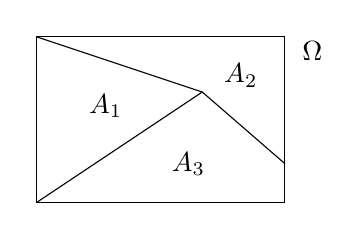
\begin{tikzpicture}[scale=0.7]
\draw (-1.5,-1.5) rectangle (3.0,1.5);
\node (O) at (3.5,1.25) {$\Omega$};
\node (v1) at (-1.5,-1.5) {};
\node (v2) at (1.5,0.5) {};
\node (v3) at (-1.5,1.5) {};
\node (v4) at (3.0,-0.8) {};
\node (a1) at (-0.25,0.25) {$A_1$};
\node (a2) at (2.2,0.8) {$A_2$};
\node (a3) at (1.25,-0.8) {$A_3$};
\draw (v1.center)--(v2.center)--(v3.center);
\draw (v4.center)--(v2.center);
\end{tikzpicture}
\end{center}

We can obtain a special case of the law of total probability which occurs frequently in problems by considering the sequence $A$, $A^c$, for some event $A$. Note that regardless of what event $A$ happens to be, this sequence always partitions $\Omega$.

\begin{corollary} If $A$ is an event with $0 < P(A) < 1$, then for any event $B$, 
$$P(B) = P(B \given A)P(A) + P(B \given A^c)P(A^c).$$
\end{corollary}

\begin{example}
If two cards are drawn from a shuffled deck, what is the probability the second card drawn is a heart?

Let $H_1 =$ `the first card is a heart' and $H_2 =$ `the second card is a heart'. We'll apply the corollary above to compute the probability of $H_2$.
$$\begin{aligned}P(H_2) &= P(H_2 \given H_1)P(H_1) + P(H_2 \given {H_1}^c)P({H_1}^c) \\ &= \frac{12}{51} \cdot \frac{1}{4} + \frac{13}{51} \cdot \frac{3}{4} = \frac{51}{204} = \frac{1}{4}\end{aligned}$$

This result makes intuitive sense. Because we're computing $P(H_2)$ in the absence of any information about the first card, we may as well have put that first card on the bottom of the deck after it's drawn without ever looking at it, so we're still drawing a card from a complete shuffled deck.
\end{example}

\begin{proof} (of Theorem \ref{lawtotalprob}) If the sequence $\{A_i\}_{i=1}^n$ partitions $\Omega$, and $B \subseteq \Omega$,
$$\begin{aligned}\Omega &= A _1 \cup A_2 \cup \, \dots \, \cup A_n \\ B \cap \Omega &= B \cap (A_1 \cup A_2 \cup \, \dots \, \cup A_n) \\ B &= (B \cap A_1) \cup (B \cap A_2) \cup \, \dots \, \cup (B \cap A_n).\end{aligned}$$

Now the sequence of events $B \cap A_1$, $B \cap A_2$, $\, \dots \,$, $B \cap A_n$ is mutually exclusive because $\{A_i\}_{i=1}^{n}$ was mutually exclusive, and this new sequence is obtained by reducing the number of outcomes in each event. The events had empty intersections initially, so removing outcomes will keep the intersections empty.
$$\begin{aligned}P(B) &= P((B \cap A_1) \cup (B \cap A_2) \cup \, \dots \, \cup (B \cap A_n)) \\ &= P(B \cap A_1) + P(B \cap A_2) + \, \cdots \, + P(B \cap A_n) \\ &= P(A_1 \cap B) + P(A_2 \cap B) + \, \cdots \, + P(A_n \cap B) \\ &= P(A_1)P(B \given A_1) + P(A_2) P(B \given A_2) + \, \cdots \, + P(A_n) P(B \given A_n)\\ &= P(B \given A_1)P(A_1) + P(B \given A_2)P(A_2)  + \, \cdots \, + P(B \given A_n)P(A_n)\end{aligned}$$
\end{proof}

\subsection*{Tree Diagrams}\index{Tree Diagram}

Tree diagrams are a nice graphical tool for organizing calculations, and have the law of total probability built in to their structure. Each column represents a step in an experiment. If we draw three balls from an urn, for example, each column will represent a draw. If we roll a die and then flip a coin, the first column will represent the roll and the second will represent the flip.

\begin{example}
What is the probability that, when three cards are drawn from a shuffled deck without replacement, exactly one heart appears?

\noindent In the tree diagram below, the three columns represent three draws from a deck of cards. When a draw results in a heart, we denote that with an $H$, and when a draw does not result in a heart, we denote that with an $N$.
\begin{center}
\begin{tikzpicture}[grow=right]
\node[bag] {.}
    child {
        node[bag] {N}        
            child {
                node[bag]{N}
                    child {
                     node[bag] {$H \qquad \frac{1482}{10200}$}
                     edge from parent
                     node[above]  {$\frac{13}{50}$}
                    }
                edge from parent
                node[below]  {$\frac{38}{51}$}
            }
            child {
                node[bag]{H}
                    child {
                     node[bag] {$N \qquad \frac{1482}{10200}$}
                     edge from parent
                     node[above]  {$\frac{38}{50}$}
                 }
                edge from parent
                node[above]  {$\frac{13}{51}$}
            }
            edge from parent 
            node[below]  {$\frac{3}{4}$}
    }
    child {
        node[bag] {H}        
        child {
            node[bag] {N}
                child {
                     node[bag] {$N \qquad \frac{1482}{10200}$}
                     edge from parent
                     node[above]  {$\frac{38}{50}$}
                 }
                edge from parent
                node[above]  {$\frac{39}{51}$}
         }
        edge from parent         
            node[above]  {$\frac{1}{4}$}
    };
\end{tikzpicture}
\end{center}

Each edge is labelled with a conditional probability. For example, the top-center edge which runs from $H$ to $N$ is labelled with $P(N_2 \given H_1)$, the probability a non-heart is drawn on the second draw, after drawing a heart on the first. Note that we only depict the branches where the desired event (`exactly one heart appears') occurs. To find the probability of this event, we simply multiply along each branch, and add the results. If $E =$ `exactly one heart is drawn', then
$$\begin{aligned}P(E) = \frac{1482}{10200} + \frac{1482}{10200} + \frac{1482}{10200} = \frac{4446}{10200} \simeq 43.6\%.\end{aligned}$$
\end{example}

This works because the branches represent mutually exclusive events (at each fork, a given trial of the experiment can proceed along only one path), so we can add the probabilities of the branches without having to appeal to the inclusion-exclusion principle. Furthermore, the intersection law states that we can compute the probability of all events along a branch occurring by multiplying their conditional probabilities. Note that if we applied the law of total probability in the above example, partitioning the sample space with $\{H_1 \cap H_2, H_1 \cap N_2, N_1 \cap H_2, N_1 \cap N_2\}$, we would obtain
$$\begin{aligned}P(E) =& \ P(E \given H_1 \cap H_2)P(H_1 \cap H_2) + P(E \given H_1 \cap N_2)P(H_1 \cap N_2) \\ &+ P(E \given N_1 \cap H_2)P(N_1 \cap H_2) + P(E \given N_1 \cap N_2)P(N_1 \cap N_2) \\
=& \ 0 + P(E \given H_1 \cap N_2)P(N_2 \given H_1)P(H_1) + P(E \given N_1 \cap H_2)P(H_2 \given N_1)P(N_1) \\ &+ P(E \given N_1 \cap N_2)P(N_2 \given N_1)P(N_1) \\
=& \ P(N_3 \given H_1 \cap N_2)P(N_2 \given H_1)P(H_1) + P(N_3 \given N_1 \cap H_2)P(H_2 \given N_1)P(N_1) \\ &+ P(H_3 \given N_1 \cap N_2)P(N_2 \given N_1)P(N_1)\end{aligned}$$
and this is exactly how we calculated the result above. Each path from left to right corresponds to a term in the sum above. The event $E$ never occurs if two hearts are drawn, so $P(E \given H_1 \cap H_2) = 0$ and that term (which corresponds to a branch not depicted in the diagram) vanishes. Although working through the notation is good practice, I expect you'll agree that in cases like this, the tree diagram is more intuitive and simplifies the calculation.

If at any point in the tree diagram, the event we're interested in is sure to occur, there's no need to continue along that branch any further.

\begin{example}
Suppose that an urn contains three red and five green balls. If three balls are drawn from the urn without replacement, what is the probability that at least one red ball will be drawn?
\tikzstyle{level 1}=[level distance=2.5cm, sibling distance=1.5cm]
\begin{center}
\begin{tikzpicture}[grow=right]
\node[bag] {.}
    child {
        node[bag] {G}        
            child {
                node[bag]{G}
                    child {
                     node[bag]{$R \qquad \frac{60}{336}$}
                     edge from parent
                     node[below]  {$\frac{3}{6}$}
                    }
                edge from parent
                node[below]  {$\frac{4}{7}$}
            }
            child {
                node[bag]{$R \qquad \frac{15}{56}$}
                edge from parent
                node[above]  {$\frac{3}{7}$}
            }
            edge from parent 
            node[below]  {$\frac{5}{8}$}
    }
    child {
        node[bag]{$R \qquad \frac{3}{8}$}        
        edge from parent         
            node[above]  {$\frac{3}{8}$}
    };
\end{tikzpicture}
\tikzstyle{level 1}=[level distance=2.5cm, sibling distance=2.25cm]
\end{center}

\noindent As soon as a red ball is drawn, there's no need to continue the branch. Regardless of what happens from that point on, a red ball will have been drawn. If A = `at least one red ball is drawn', then 
$$\begin{aligned}P(A) = \frac{3}{8} + \frac{15}{56} + \frac{60}{336} = \frac{276}{336} \simeq 82.1\%.\end{aligned}$$
\end{example}

\begin{example}
Suppose we draw cards with replacement from a shuffled deck until the first ace appears. What is the probability that all cards drawn are black?

\tikzstyle{level 1}=[level distance=2.5cm, sibling distance=1.5cm]
\begin{center}
\begin{tikzpicture}[grow=right]
\node[bag] {.}
    child {
        node[bag] {BNA}        
            child {
                node[bag]{BNA}
                    child {
                     node[bag]{$\dots$}
                     edge from parent
                     node[below]  {$\frac{24}{52}$}
                    }
										child {
                     node[bag]{$BA$}
                     edge from parent
                     node[above]  {$\frac{2}{52}$}
                    }
                edge from parent
                node[below]  {$\frac{24}{52}$}
            }
            child {
                node[bag]{$BA$}
                edge from parent
                node[above]  {$\frac{2}{52}$}
            }
            edge from parent 
            node[below]  {$\frac{24}{52}$}
    }
    child {
        node[bag]{$BA$}        
        edge from parent         
            node[above]  {$\frac{2}{52}$}
    };
\end{tikzpicture}
\tikzstyle{level 1}=[level distance=2.5cm, sibling distance=2.25cm]
\end{center}

Here $BA$ denotes `black ace' and $BNA$ denotes `black non-ace'. There's no limit to the number of draws that could occur before the first black ace appears, so the tree diagram is infinite. However, we can still sum the products along each branch. Let $OB = $ `only black cards are drawn', then
$$\begin{aligned}P(OB) &= \frac{2}{52} + \frac{24}{52}\cdot\frac{2}{52} + \frac{24}{52}\cdot\frac{24}{52}\cdot\frac{2}{52} +  \frac{24}{52}\cdot\frac{24}{52}\cdot\frac{24}{52}\cdot\frac{2}{52} + \ \dots \\
&= \frac{2}{52}\left(1 + \frac{24}{52} + \left(\frac{24}{52}\right)^2 + \left(\frac{24}{52}\right)^3 + \ \dots\right) \\
&= \frac{2}{52}\left(\sum_{i=0}^{\infty} \left(\frac{24}{52}\right)^n\right) \\
&= \frac{2}{52} \cdot \frac{1}{1-(\frac{24}{52})} = \frac{1}{14} \simeq 7.1\%\end{aligned}$$
\end{example}

Note that the sum of the infinite series above was evaluated with the geometric series sum formula, $a+ar+ar^2+ \dots = \frac{a}{1-r}$ when $-1 < r < 1$.

\section{Independence}\label{IndependentEventsSec}

Suppose we flip a coin and then roll a die. Let $H =$ `a head is flipped', $E =$ `an even number is rolled' and $L =$ `a number larger than three was rolled'. Note that
$$P(E) = \frac{1}{2} \text{ \ and \ } P(E \given H) = \frac{1}{2}$$
since knowing that a head was flipped doesn't change the probability an even number is rolled. On the other hand, we can calculate 
$$P(E) = \frac{1}{2} \text{ \ and \ } P(E \given L) = \frac{2}{3}.$$
In this case, knowledge that the number rolled was a four, five, or six increases the probability that the result of the roll was even. The events $E$ and $H$ are said to be \emx{independent}, while the events $E$ and $L$ are \emx{not independent}.

\begin{definition}\label{independentevents}
Events $A$ and $B$ are called \newterm{independent}\index{Events!Independent}\index{Independence!of a pair of Events} if $P(B) = P(B \given A)$.
\end{definition}

\begin{example}Suppose we flip a coin two times. Note that $\Omega = \{HH, HT, TH, TT\}$ is a sample space with equally likely outcomes for the experiment.

If we consider the events $H_1 =$ `the first flip is a head' and $H_2 =$ `the second flip is a head', then $P(H_2) = \frac{1}{2}$ and $P(H_2 \given H_1) = \frac{1}{2}$, so these events are independent.

If we instead let $H_1 =$ `the first flip is a head' and $T_1 =$ `the first flip is a tail', then $P(T_1) = \frac{1}{2}$ and $P(T_1 \given H_1) = 0$, so these two events are not independent.
\end{example}

\begin{example}
Consider two cards drawn from a shuffled deck. Let $S_1 =$ `a spade is drawn on the first draw' and $S_2 =$ `a spade is drawn on the second draw'. Then $S_1$ and $S_2$ are independent provided the draws are done with replacement, but not independent if the draws are done without replacement. In this second case, $P(S_2 \given S_1) = \frac{12}{51}$, but using the law of total probability, $P(S_2) = \frac{1}{4}$.
\end{example}

Using the definition of the conditional probability $P(A \given B)$, we can state what it means for two events to be independent in a different way. 
$$P(A) = P(A \given B) \biimp P(A) = \frac{P(A \cap B)}{P(B)} \biimp P(A)P(B) = P(A \cap B)$$
Thus, when $A$ and $B$ are independent events, $P(A \cap B) = P(A)P(B)$. This relation is often used as the definition of independence. As we just saw, it's equivalent to the definition we gave earlier but also applies when $P(A) = 0$ or $P(B) = 0$ (in these cases $P(A\given B)$ or $P(B \given A)$ would be undefined).

\begin{keypoint}
Independence is a symmetric relation, which you can interpret intuitively as `the probability of one event occurring is not influenced by the occurrence of the other' without worrying about which event comes first. The alternate form of the definition $P(A \cap B)=P(A)P(B)$ confirms this, as swapping the roles of $A$ and $B$ yields the same equation.
\end{keypoint}

\begin{theorem}\label{compindependent}
If $A$ and $B$ are independent, then $A$ and $B^c$ are independent.
\end{theorem}
\begin{proof}
Note that $A = (A \cap B) \cup (A \cap B^c)$ and hence $P(A) = P(A \cap B) + P(A \cap B^c)$ since the two events on the right are mutually exclusive. Isolating $P(A \cap B^c)$,
$$\begin{aligned}P(A \cap B^c) &= P(A) - P(A \cap B) \\
&= P(A) - P(A)P(B) \\
&=P(A)(1-P(B)) \\
&= P(A)P(B^c).\end{aligned}$$
\end{proof}

\begin{corollary}
If $A$ and $B$ are independent, then $A^c$ and $B^c$ are independent.
\end{corollary}
\begin{proof}
If $A$ and $B$ are independent, then $A$ and $B^c$ are independent by Theorem \ref{compindependent}, but independence is symmetric, so applying Theorem \ref{compindependent} again, this time to $B^c$ and $A$, we conclude $B^c$ and $A^c$ are independent.
\end{proof}

\begin{remark}
The upshot of the previous theorem and its corollary is that the independence relation is unaffected by complements. This can be useful, since calculating $P(A^c \given B)$, or $P(A \given B^c)$, or $P(A^c \given B^c)$ may be easier than calculating $P(A \given B)$.
\end{remark}

Given a sequence of events $\{A_i\}_{i=1}^{n}$, we say this sequence is independent if the occurrence of any collection of these events does not influence the chance that any other event in the sequence occurs. Formally, it's easiest to state this by extending the relation $P(A \cap B) = P(A)P(B)$ as below.

\begin{definition}\index{Independence!of a sequence of Events}
The sequence of events $\{A_i\}_{i=1}^{n}$ is independent if for any subsequence $A_{i_1}, A_{i_2}, \, \dots \, , A_{i_k}$ of events taken from $\{A_i\}_{i=1}^{n}$,
$$\begin{aligned}P(A_{i_1} \cap A_{i_2} \cap \, \dots \, \cap A_{i_k}) = P(A_{i_1})P(A_{i_2}) \, \cdots \, P(A_{i_k})\end{aligned}$$
\end{definition}

\begin{example}
Suppose we toss a fair coin twice. Let $H_1 =$ `The first toss is heads', $H_2 =$ `The second toss is heads', and $E =$ `Exactly one toss results in heads'. As we already observed, $H_1$ and $H_2$ are independent. Moreover, $P(E) = \frac{1}{2}$ since exactly one head is flipped in two of the four equally likely outcomes, and $P(E \given H_1) = \frac{1}{2}$ since assuming $H_1$ occurs, $E$ occurs when the second flip is a tail. Thus, $H_1$ and $E$ are independent, and essentially the same argument shows $H_2$ and $E$ are independent.

Since each pair of events in the sequence $\{H_1, H_2, E\}$ is independent, we say this sequence is pairwise independent\index{Pairwise Independence}. However, note that if we assume both $H_1$ and $H_2$ occur, the probability $E$ occurs becomes zero, that is, $P(H_1 \cap H_2 \cap E) = 0$, but we can calculate $P(H_1)P(H_2)P(E) = \frac{1}{2}\cdot\frac{1}{2}\cdot\frac{1}{2} = \frac{1}{8}$.
\end{example}

The example above illustrates that even if every pair of events in a sequence is independent, there could still be some event in the sequence whose probability is influenced by the joint occurrence of some larger collection of other events. In other words, for sequences of events, pairwise independence does not imply independence.

\begin{example}
Suppose that a 64 bit sequence (a sequence of 64 zeros and ones) is sent over an unreliable channel. The probability that each bit gets flipped is 0.005 independent of what happens to the other bits. What is the probability that the entire sequence is received without errors?

Let $F_i = $ `the $i^{th}$ bit gets flipped', then $P(F_i) = 0.005$, and the probability that the $i^{th}$ bit is received correctly is $P({F_i}^c) = 1-0.005 = 0.995$. If $E =$ `the entire string is received without any flipped bits' then
$$\begin{aligned}P(E) &= P({F_1}^c \cap {F_2}^c \cap \, \dots \, \cap {F_{64}}^c) \\
&= P({F_1}^c)P({F_2}^c) \, \cdots \, P({F_{64}}^c) \\
&= 0.995 \cdot 0.995 \cdot \, \cdots \, \cdot 0.995 \\
&\simeq 0.72556 \simeq 72.6\%\end{aligned}$$
\end{example}





